\section{Descarte de las causas del lugar}\label{sec:descarte}

\subsection{Clima y altitud}\label{sec:clima}

Las variables que más difieren entre regímenes son climáticas (Tabla~\ref{tab:clima}). Para medir cuánto de la brecha
podrían explicar, estimamos su efecto dentro de los regímenes con una regresión que controla por régimen, y lo
multiplicamos por la diferencia entre regímenes. Ninguna explica más de 0.11 de las 1.44\,t/ha, y ningún efecto es
significativo. La altitud media casi no cambia: 2690\,m en A y 2638\,m en B.

\begin{table}[t]
\centering
\caption{Variables con mayor diferencia entre regímenes}
\label{tab:clima}
\footnotesize
\begin{tabular}{@{}lrrrr@{}}
\toprule
Variable & Dif.\ A$-$B & Efecto & $p$ & Brecha \\
 & (desv.) & (t/ha/desv.) & & (t/ha) \\
\midrule
Anomalía de lluvia en siembra & $-1.76$ & $-0.064$ & 0.42 & 0.11 \\
Lluvia en siembra & $-1.64$ & $-0.066$ & 0.34 & 0.11 \\
Amplitud térmica & $-1.64$ & $-0.053$ & 0.44 & 0.09 \\
Anomalía de Tmax, may--sep & $1.59$ & $0.049$ & 0.45 & 0.08 \\
\midrule
Brecha observada & & & & 1.44 \\
\bottomrule
\end{tabular}
\end{table}

El experimento natural de Singuilucan es más claro (Tabla~\ref{tab:zonas}). Singuilucan tiene la misma temperatura
mínima y la misma amplitud térmica que el régimen A, más lluvia y un cultivo igual de verde o más, y aun así rinde
como el B del sur. El clima no puede ser la causa.

\begin{table}[t]
\centering
\caption{Medianas por zona. B norte es Singuilucan}
\label{tab:zonas}
\footnotesize
\begin{tabular}{@{}lrrr@{}}
\toprule
 & A & B norte & B sur \\
\midrule
Rendimiento (t/ha) & 4.52 & \textbf{3.20} & 3.00 \\
Tmin may--sep (°C) & 14.0 & \textbf{14.0} & 13.0 \\
Amplitud térmica (°C) & 9.6 & 9.8 & 10.6 \\
Lluvia may--oct (mm) & 899 & \textbf{1262} & 884 \\
NDVI máximo, Planet & 0.72 & \textbf{0.79} & 0.74 \\
Verdor acumulado en el pico & 14.3 & \textbf{15.7} & 14.8 \\
Duración del verdor (días) & 152 & 119 & 133 \\
\bottomrule
\end{tabular}
\end{table}

\subsection{Fenología y verdor}\label{sec:fenologia}

La única diferencia real que encontramos en el satélite está en el calendario del cultivo. Según la serie de Planet,
el régimen A emerge alrededor del 6 de junio y el B del 16 de junio, y el verdor del A dura hasta el 6 de noviembre,
contra el 26 de octubre del B. Esto coincide con la recomendación técnica de sembrar las variedades tardías hasta el
10 de junio y las precoces en la segunda quincena de junio~\cite{inifap_hgo}. Un ciclo más largo da más tiempo de
llenado de grano, así que la hipótesis tiene sentido agronómico.

Sin embargo, no pasa la segunda prueba (Fig.~\ref{fig:fenologia}). Dentro del régimen A, las 35 parcelas que
emergieron después del 7 de junio rinden 4.47\,t/ha y las 52 tempranas, 4.50. Dentro de cada régimen, la correlación
del rendimiento con la fecha de emergencia, la duración del ciclo o el NDVI máximo está entre $-0.15$ y $0.25$.
Tepeapulco emerge tan tarde como Singuilucan y rinde 4.45 contra 3.08. El régimen A rinde alrededor de 4.5\,t/ha sin
importar cuándo se sembró.

\begin{figure}[t]
\centering
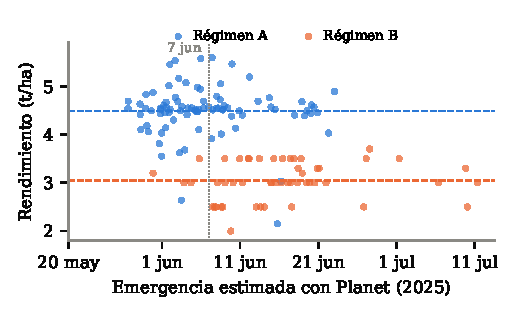
\includegraphics[width=\columnwidth]{r3_fenologia}
\caption{Rendimiento contra fecha de emergencia. Las líneas punteadas son la media de cada régimen. La siembra tardía
no baja el rendimiento del régimen A.}
\label{fig:fenologia}
\end{figure}

\subsection{Suelo}\label{sec:suelo}

El suelo era el mejor candidato restante, porque actúa parejo sobre toda una zona y no viene en los datos del reto.
La literatura señalaba el tepetate (fase dúrica) de los Llanos de Apan como limitante. Asignamos a cada parcela la
unidad de suelo que ocupa la mayor parte de su superficie en la carta de INEGI.

Si el suelo causara la brecha, se cumplirían dos cosas. Primero, dentro de un mismo régimen las parcelas con suelos
distintos rendirían distinto. Segundo, las parcelas con el mismo suelo rendirían parecido aunque fueran de distinto
régimen, y la brecha desaparecería. No se cumple ninguna (Fig.~\ref{fig:suelo}):
\begin{itemize}
\item \textbf{Distinto suelo, mismo rendimiento.} En el régimen A, los cinco grupos de suelo rinden entre 4.33 y
4.56\,t/ha. En el B, el Phaeozem y el Umbrisol rinden 3.05 y 3.02. Cambiar de suelo no mueve el rendimiento.
\item \textbf{Mismo suelo, la misma brecha.} Al comparar parcelas con el mismo suelo, la brecha entre regímenes sigue
entre 1.45 y 1.77\,t/ha, igual que la brecha total de 1.44. Hay dos unidades presentes en ambos regímenes. En el
Phaeozem con Durisol, Almoloya (A) rinde 4.63 y Calpulalpan y Emiliano Zapata (B) rinden 3.08. En el Umbrisol con
Vertisol, Cuautepec (A) rinde 4.68 y Singuilucan (B) rinde 2.91.
\item \textbf{El tepetate no está donde haría falta.} Es más común en el régimen A que en el B (53 parcelas contra
27), y en el A rinde 4.45, igual que sin tepetate.
\end{itemize}
Si el suelo fuera la causa, los puntos de la Fig.~\ref{fig:suelo} se agruparían por suelo. En cambio, se agrupan por
régimen: todo el azul cerca de 4.5 y todo el naranja cerca de 3, sea cual sea el suelo. La carta de INEGI es
1:250\,000, así que describe el suelo dominante de unidades de varios kilómetros cuadrados y no el de cada parcela.
Una diferencia de suelo más fina no se puede descartar con este mapa, pero tendría que seguir exactamente la frontera
entre municipios.

\begin{figure}[t]
\centering
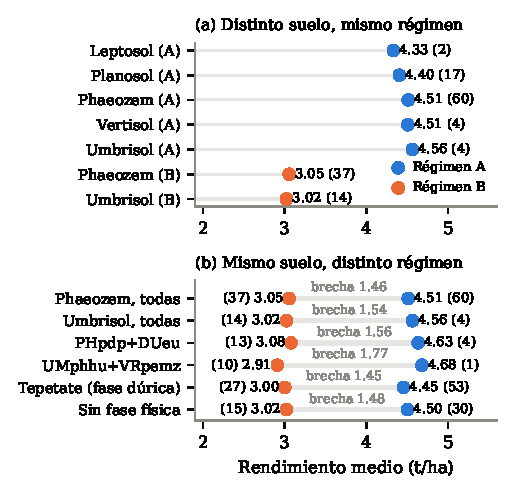
\includegraphics[width=\columnwidth]{r4_suelo}
\caption{Rendimiento medio por suelo y régimen, con el número de parcelas entre paréntesis. (a) Dentro de cada
régimen, el suelo no cambia el rendimiento. (b) Con el mismo suelo, la brecha entre regímenes sigue siendo de 1.5\,t/ha.
PHpdp+DUeu y UMphhu+VRpemz son las dos unidades que aparecen en ambos regímenes.}
\label{fig:suelo}
\end{figure}

\subsection{Ceniza del Popocatépetl}\label{sec:volcan}

Los municipios B del sur son los más cercanos al volcán (60 a 68\,km), y en enero de 2025 Cenapred reportó caída de
ceniza en Calpulalpan y Nanacamilpa~\cite{ceniza_ene25}. Tres hechos descartan esta causa. Primero, Singuilucan es el
municipio más lejano (106\,km) y rinde como B (Fig.~\ref{fig:volcan}). Además, a esa distancia una nube de ceniza mide
decenas de kilómetros de ancho y no distingue parcelas a 9\,km entre sí. Segundo, la ceniza de enero cayó antes de la
siembra, y de mayo a octubre de 2025 los pronósticos dirigían la ceniza al oeste y suroeste, lejos de la
zona~\cite{ceniza_2025}. Tercero, la ceniza daña al cultivo reduciendo su área foliar y adelantando la
senescencia~\cite{ligot2023}, pero el régimen B tiene igual o más verdor que el A.

\begin{figure}[t]
\centering
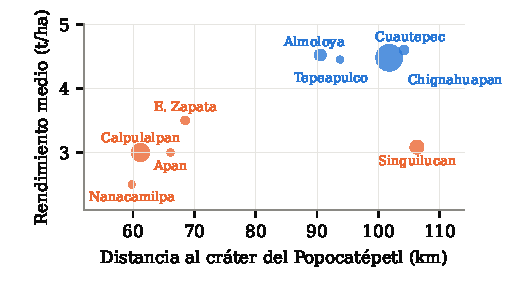
\includegraphics[width=\columnwidth]{r5_volcan}
\caption{Rendimiento medio por municipio contra la distancia al cráter. El tamaño indica el número de parcelas.}
\label{fig:volcan}
\end{figure}
